A seguir, são apresentadas perspectivas teóricas relevantes para o contexto do presente
trabalho.
\section{Sensoriamento remoto}
O sensoriamento remoto é uma área fundamental em vários campos científicos e tecnológicos. Ele pode ser definido  como:
\begin{quote}
"A arte ou ciência de dizer algo sobre um objeto sem tocá-lo." \parencite[{p. 34}]{fischer1976}
\end{quote}

Ao longo dos anos, o sensoriamento remoto tem evoluído, proporcionando uma variedade de aplicações em diversas áreas. Uma visão geral da evolução do sensoriamento remoto pode ser observada na Tabela \ref{tab:evolucao_sr}

\begin{table}[!htb]
\caption{Evolução do sensoriamento remoto.} \label{tab:evolucao_sr}
\begin{tabularx}{\textwidth}{|c|X|} \hline
\textbf{Ano} & \textbf{Evento} \\ \hline
1800         & Descoberta do infravermelho por Sir William Herschel. \\ \hline
1839         & Início da prática da fotografia. \\ \hline
1847         & Espectro infravermelho mostrado por A. H. L. Fizeau e J. B. L. Foucault para compartilhar propriedades com a luz visível. \\ \hline
1850-1860    & Fotografia a partir de balões. \\ \hline
1873         & Teoria da energia eletromagnética desenvolvida por James Clerk Maxwell. \\ \hline
1909         & Fotografia a partir de aviões. \\ \hline
1914-1918    & Primeira Guerra Mundial: reconhecimento aéreo. \\ \hline
1920-1930    & Desenvolvimento e aplicações iniciais da fotografia aérea e fotogrametria. \\ \hline
1929-1939    & Depressão econômica gera crises ambientais que levam a aplicações governamentais da fotografia aérea. \\ \hline
1930-1940    & Desenvolvimento de radares na Alemanha, Estados Unidos e Reino Unido. \\ \hline
1939-1945    & Aplicações da Segunda Guerra Mundial de porções não visíveis do espectro eletromagnético. \\ \hline
1950-1960    & Pesquisa e desenvolvimento militares. \\ \hline
1956         & Pesquisa de Colwell sobre detecção de doenças de plantas com fotografia infravermelha. \\ \hline
1960-1970    & Primeiro uso do termo sensoriamento remoto, satélite meteorológico TIROS. \\ \hline
1972         & Lançamento do Landsat 1. \\ \hline
1970-1980    & Avanços rápidos no processamento digital de imagens. \\ \hline
1980-1990    & Landsat 4: nova geração de sensores Landsat. \\ \hline
1980s        & Desenvolvimento de sensores hiperespectrais. \\ \hline
1990s        & Sistemas globais de sensoriamento remoto, lidares. \\ \hline
2000s        & Lançamento dos satélites Terra e Aqua da NASA para monitoramento climático. \\ \hline
2010s        & Lançamento dos satélites Sentinel pelo programa Copernicus da ESA. \\ \hline
\end{tabularx}
\fonte{Retirado de \textcite{campbell2011}.}
\end{table}

Uma das áreas de aplicação do sensoriamento remoto na atualidade é a agricultura. Estudos recentes, como o de \textcite{weiss2020}, destacam sua importância na adaptação e evolução das práticas agrícolas. Eles fornecem informações repetitivas sobre o estado das culturas ao longo da safra, em diferentes escalas e para diferentes partes interessadas.

As pesquisas ressaltam suas vantagens na monitorização das culturas, estimativa de produtividade e tomada de decisão em diferentes estágios da produção agrícola \parencite{shanmugapriya2019, khanal2020}. Entre esses benefícios, destacam-se a capacidade de monitorar vastas extensões de terra de maneira rápida e eficaz, a obtenção de informações em tempo real e a habilidade de integrar dados oriundos de diversas fontes para análises mais abrangentes.

Além disso, estudos evidenciam seu papel na obtenção de estatísticas agrícolas, contribuindo para a definição de unidades amostrais, estratificação e alocação de amostras \parencite{carfagna2005}. Essa contribuição é viabilizada pela integração de análise de imagens de satélite e dados de sensores, permitindo estimar com precisão a área plantada e a produtividade das culturas. Isso fornece subsídios essenciais para a formulação de políticas públicas e embasamento na tomada de decisões estratégicas no âmbito agrícola.

\subsection{Telemetria}
A telemetria é um campo complementar ao sensoriamento remoto e é definida como:
\begin{quote}
"A indicação, registro ou integração de uma quantidade em um ponto remoto por meios eleitorais e de tradução métrica.  Grandezas de estados elétricos ou mecânicos estão normalmente envolvidas, embora existam outras aplicações diversas para telemedição." \parencite[{p. 3}]{telemetering1941}
\end{quote}

De acordo com \textcite{telemetry_systems2002}, ao longo das décadas, os sistemas de telemetria evoluiram gradativamente, impulsionada por avanços tecnológicos em eletrônica, comunicações e processamento de dados. Inicialmente, a telemetria era predominantemente utilizada em aplicações aeroespaciais e militares para monitorar o \textit{status} e o desempenho de aeronaves e foguetes. 

Com o passar do tempo, sua aplicabilidade se expandiu para uma variedade de setores, incluindo medicina, indústria automotiva, energia e telecomunicações \parencite{Lizhuang_telemetry2021, Hassanien2020, Ding_telemetry2017}.

Para \textcite{Lizhuang_telemetry2021}, os avanços na miniaturização de sensores e no aumento da capacidade de armazenamento de dados possibilitaram a coleta de uma quantidade crescente de dados de telemetria. Além disso, melhorias nas técnicas de transmissão de dados têm aprimorado a análise dessas informações. 

\textcite{Ding_telemetry2017} afirmam que o desenvolvimento de algoritmos de análise de dados e inteligência artificial (IA) tem permitido uma compreensão mais profunda dos padrões e tendências nos dados telemétricos. Isso tem levado a aprimoramentos em diversos processos e sistemas.

Neste trabalho, a telemetria é empregada para monitorar variáveis ambientais, tais como umidade do solo, temperatura e umidade relativa do ar, em uma área de cultivo.  Os dados são coletados por sensores remotos e transmitidos através de protocolos de comunicação. Os protocolos de comunicação usadas neste projeto foram o Transporte de Telemetria de Enfileiramento de Mensagens - MQTT (sigla do inglês, \textit{Message Queuing Telemetry Transport}) e o Protocolo de Transferência de Hipertexto - HTTP (sigla do inglês, \textit{Hypertext Transfer Protocol}) para um servidor remoto (\textit{broker}).

\section{Sistemas embarcados}
Há várias concepções propostas para sistemas embarcados; um conceito geral pode ser definido como:

\begin{quote}
"Aquele que possui \textit{hardware} de computador com \textit{software} embutido como um de seus componentes mais importantes. É um sistema baseado em computador dedicado para uma ou várias aplicações. Pode ser um sistema independente ou parte de um sistema maior." \parencite[{p. 39}]{dutta2014comprehensive}
\end{quote}

Sua utilização abrange desde dispositivos simples, como controles remotos e eletrodomésticos, até sistemas complexos, como veículos autônomos e equipamentos médicos \parencite{lee2008cyber, kato2018autoware}. Eles desempenham um papel fundamental na automação de processos industriais, na monitoração e controle de dispositivos, na coleta e processamento de dados em tempo real, entre outras funções \parencite{dutta2014comprehensive}.

Os sistemas embarcados são compostos por diversos componentes, incluindo microcontroladores, sensores, atuadores, interfaces de comunicação e \textit{software} embarcado \parencite{lee2008cyber}.
Eles são projetados para atender a requisitos específicos de desempenho, consumo de energia, tamanho e custo, dependendo da aplicação \parencite{Mazid_microcontrolador2011}.

Na seção seguinte, serão abordados os microcontroladores e sua importância na implementação de soluções embarcadas.

\section{Microcontroladores}

Segundo \textcite{lee2008cyber}, os microcontroladores são componentes essenciais dos sistemas embarcados. Estes desempenham um papel central na execução de tarefas específicas e no controle de dispositivos em uma variedade de aplicações. Ele é composto por:

\begin{quote}
  "Um microprocessador (CPU), além de uma quantidade fixa de memória principal (RAM), memória de programa (ROM/Flash),  interfaces de entrada/saída (I/O), temporizadores e conversores analógico-digitais (ADC), todos em um único chip." \parencite[{p. 40}]{Mazid_microcontrolador2011}
\end{quote}

A Tabela \ref{tab:evolucao_microcontroladores} mostra alguns modelos de microcontroladores e suas finalidades, desde modelos antigos até os mais recentes. Neste trabalho, o principal motivo da escolha do microcontrolador ESP32 se deu em razão de sua capacidade de comunicação \textit{wireless} embutida. Esse recurso também é nativo em outros microcontroladores como Raspberry Pi 4, porém, o ESP32 se destaca por um menor custo e consumo de energia \parencite{ESP32_usage}.

\begin{table}[!htb]
\caption{Evolução dos microcontroladores.} \label{tab:evolucao_microcontroladores}
\begin{tabularx}{\textwidth}{|c|c|c|X|} \hline
\textbf{Modelo} & \textbf{Ano de Lançamento} & \textbf{Preço (USD)} & \textbf{Componentes Embutidos} \\ \hline
Intel 8051 & 1977 & \$1 - \$2 & CPU de 8 bits, memória RAM e ROM integradas, temporizador, portas de I/O \parencite{8051_usage}. \\ \hline
PIC16F84A & 1993 & \$2 - \$4 & CPU de 8 bits, memória flash e RAM integradas, temporizador, portas I/O \parencite{PIC16F84A_usage}. \\ \hline
Arduino Uno & 2010 & \$3 - \$4 & CPU de 8 bits, memória flash e RAM integradas, temporizador, portas I/O digitais, USB \parencite{Arduino_usage}. \\ \hline
STM32F4 & 2011 & \$20 - \$25 & CPU de 32 bits, memória flash e RAM integradas, temporizador, interfaces SPI, UART, I2C \parencite{STM32F4_usage}. \\ \hline
ESP32 & 2016 & \$3 - \$4 & CPU de 32 bits, \textit{Wi-Fi} e \textit{Bluetooth} integrados, memória flash e RAM integradas, temporizador, portas GPIO, SPI, UART, I2C \parencite{ESP32_usage}. \\ \hline
Raspberry Pi 4 & 2019 & \$55 - \$60 & CPU de 64 bits, memória RAM integrada, Ethernet, Wi-Fi, portas USB, HDMI, GPIO \parencite{RaspberryPi4_usage}. \\ \hline
\end{tabularx}
\fonte{Elaborado pelo autor, 2024.}
\end{table}

A seguir, serão discutidas as características do ESP32 e sua relevância  na implementação de sistemas de monitoramento e controle.

\subsection{ESP32}

O ESP32 é um microcontrolador de baixo custo desenvolvido pela Espressif Systems. De acordo com \textcite{ESP32_usage}, este componente é amplamente utilizado em projetos de Internet das Coisas - IoT (sigla do inglês, \textit{Internet of Things}) devido às suas capacidades de conexão integradas e poder de processamento.

Baseado em um microprocessador \textit{dual-core} Tensilica Xtensa LX6, o ESP32 opera em frequências de até 240 MHz, apresentando uma arquitetura de 32 bits. Além disso, possui uma variedade de periféricos (Tabela \ref{tab:esp32_perifericos}) o que o torna versátil para uma variedade de aplicações \parencite{EspressifESP32}.

Uma das principais vantagens do ESP32, como destacado por \textcite{ESP32_usage}, é sua capacidade de conexão Wi-Fi e Bluetooth embutida, suportando os padrões 802.11 b/g/n Wi-Fi, Bluetooth 4.2 e Bluetooth Low Energy (BLE). Isso possibilita a comunicação sem fio em ambientes de IoT.

O ESP32 pode ser programado usando o Arduino IDE e o ESP-IDF (Espressif IoT Development Framework), ambos baseados em C/C++. Através dessas plataformas (IDEs), os desenvolvedores podem acessar os recursos do ESP32 e criar aplicações. Esses projetos vão desde simples automações residenciais até dispositivos complexos de monitoramento \parencite{ferrandez2018precision, junior2022data, hsu2020creative}.

Neste trabalho, o ESP32 atua como um ponto de controle, permitindo a comunicação bidirecional entre o mundo físico (representado pelas variáveis ambientais) e o mundo digital (representado pelo \textit{broker}). Essa capacidade de interação direta entre \textit{hardware}, \textit{software} e o ambiente físico exemplifica a definição de um Sistema Cyberfísico - CPS (sigla do inglês, \textit{Cyber-Physical System}), como será abordado na próxima subseção.

\begin{table}[!htb]
  \caption{Periféricos do microcontrolador ESP32} \label{tab:esp32_perifericos}
  \begin{tabularx}{\textwidth}{|c|X|X|} \hline
    \textbf{Abreviação} & \textbf{Significado} & \textbf{Função} \\ \hline
    GPIO & Entrada/saída de uso geral. & Permite a comunicação de propósito geral com dispositivos externos através de sinais de entrada e saída digitais.  \\ \hline
    UART & Receptor/transmissor assíncrono universal. & Facilita a comunicação serial assíncrona entre o microcontrolador e outros dispositivos, como sensores e módulos de comunicação. \\ \hline
    SPI & Interface periférica serial. & Permite a comunicação serial síncrona de alta velocidade entre o microcontrolador e dispositivos periféricos, como sensores, displays e memórias. \\ \hline
    I2C & Circuito Interintegrado. & Oferece uma interface serial de dois fios para comunicação entre vários dispositivos. \\ \hline
  \end{tabularx}
  \fonte{Adaptado de \textcite{EspressifESP32}.}
\end{table}

\section{Sistemas cyberfísicos}

Os sistemas CPSs representam uma evolução dos sistemas embarcados. Eles podem ser definidos como:

\begin{quote}
"Integrações de computação com processos físicos. Computadores embarcados e redes que monitoram e controlam os processos físicos, geralmente com \textit{loops} de \textit{feedback} onde os processos físicos afetam as computações e vice-versa." \parencite[{p. 363}]{lee2008cyber}
\end{quote}

Recentemente, tem havido uma tendência crescente no uso de CPSs em aplicações práticas na agricultura. Por exemplo, \textcite{ahmad2020smart} demonstraram um sistema de monitoramento inteligente que utiliza abordagens para rastrear o comportamento e as atividades de roedores no campo. O sistema auxilia especialistas em controle de pragas e agricultores na aplicação mais eficiente de métodos de controle tradicionais.

Da mesma forma, \textcite{rad2015smart} propuseram um modelo de arquitetura de CPS para o monitoramento de culturas de batata, resultando na melhoria da produtividade. \textcite{rijswijk2021digital} discutiram o papel dos sistemas socio-cyberfísicos (SCPSs) na transformação digital da agricultura e das áreas rurais. Eles destacaram a necessidade de compreender as relações entre os aspectos sociais e tecnológicos para uma aplicação bem-sucedida.

O presente trabalho se enquadra na categoria de CPS, pois integra componentes físicos, computacionais e de comunicação. Seu papel é monitorar um processo físico (a irrigação) de maneira automatizada e em tempo real. A infraestrutura necessária para conectar dispositivos físicos à internet e entre si é definida como IoT, como será abordado na próxima subseção. 

\section{Internet das coisas}
A IoT é um campo multidisciplinar que se desenvolveu ao longo do tempo, com contribuições de diversas áreas. \textcite{datta2017} representa esse campo como um \textit{"tsunami"}, que começa com a exploração marítima, seguida pelo desenvolvimento da engenharia, passando pela automação, eletricidade, sensoriamento, e culminando na IoT (Figura \ref{figura:evolucao_iot}). 

Cada uma dessas etapas representa um avanço na integração de tecnologia e comunicação, resultando em um sistema interconectado e inteligente. A exploração marítima marcou o início do uso de tecnologias para navegação e comunicação a longas distâncias. Com a engenharia, foram estabelecidas as bases para a construção de infraestruturas complexas e sistemas mecânicos. 

A automação trouxe a capacidade de controlar processos e máquinas de forma eficiente, enquanto os avanços na eletricidade permitiram a disseminação de dispositivos eletrônicos. O sensoriamento adicionou a capacidade de monitorar e coletar dados em tempo real, preparando o terreno para a IoT, onde todos esses elementos se unem para criar um ambiente altamente conectado e responsivo.

A IoT pode ser definida como:

\begin{quote}
"Um paradigma emergente de objetos cotidianos que, através da interação com o ambiente e com outros dispositivos, coletam e compartilham dados, geralmente utilizando protocolos de comunicação padronizados e interoperáveis, e, em alguns casos, interagindo com usuários ou outros dispositivos." \parencite[{p. 44}]{kortuem2009things}
\end{quote}

Segundo \textcite{minerva2015towards}, a ideia de IoT foi proposta pela primeira vez por \textcite{ashton1999things}. Ele argumentou que poderia revolucionar a maneira como interage-se com o mundo físico, permitindo que artefatos se comuniquem entre si e com sistemas de computador.

Ao longo dos anos 2000, avanços em tecnologias de comunicação sem fio, sensores e sistemas embarcados possibilitaram o desenvolvimento prático da IoT, como destacado por \textcite{kortuem2009things}. Na década de 2010, a IoT começou a ganhar notoriedade em uma variedade de setores, incluindo saúde, manufatura, transporte e agricultura. Vários autores discutiram como essas tecnologias abriram caminho para a criação de redes de dispositivos interconectados em diversos campos \parencite{kortuem2009things, tan2010things, minerva2015towards}.

Atualmente, a IoT continua a evoluir, com o surgimento de novas tecnologias como a computação em névoa, termo conhecido em inglês como \textit{fog computing}, e integrações com inteligências artificiais (IAs) \parencite{junior2022data}. Na agricultura, a IoT é empregada para melhorar a eficiência e produtividade.

O estudo conduzido por \textcite{ferrandez2018precision} exemplifica o uso da IoT para otimizar os processos agrícolas. Através de sensores interconectados, demonstrou-se ser possível monitorar uma série de variáveis físicas, como a umidade do solo, a temperatura e a umidade relativa do ar. Essa abordagem mostrou-se promissora, capacitando os agricultores a tomarem decisões mais embasadas em relação ao momento ideal para o plantio, à irrigação e à aplicação de fertilizantes.

Combinada à computação em névoa, a IoT possibilita o processamento local dos dados coletados pelos sensores, o que reduz o tempo de resposta e os custos associados ao envio e recebimento de dados \parencite{hsu2020creative}. Além disso, a integração com a IA permite a análise preditiva e a otimização desses sistemas, fornecendo informações que aumentam a produtividade e diminuem o desperdício.

Para facilitar a comunicação entre dispositivos, servidores e outros sistemas, o presente trabalho utilizou os protocolos HTTP e MQTT. Esses protocolos permitem o acesso remoto e o controle dos dispositivos conectados à IoT, como será abordado nas próximas subseções.

\begin{figure}[!htb] \centering
  \caption{\textit{"Tsunami"} da IoT} \label{figura:evolucao_iot}
  \begin{varwidth}{\linewidth}
    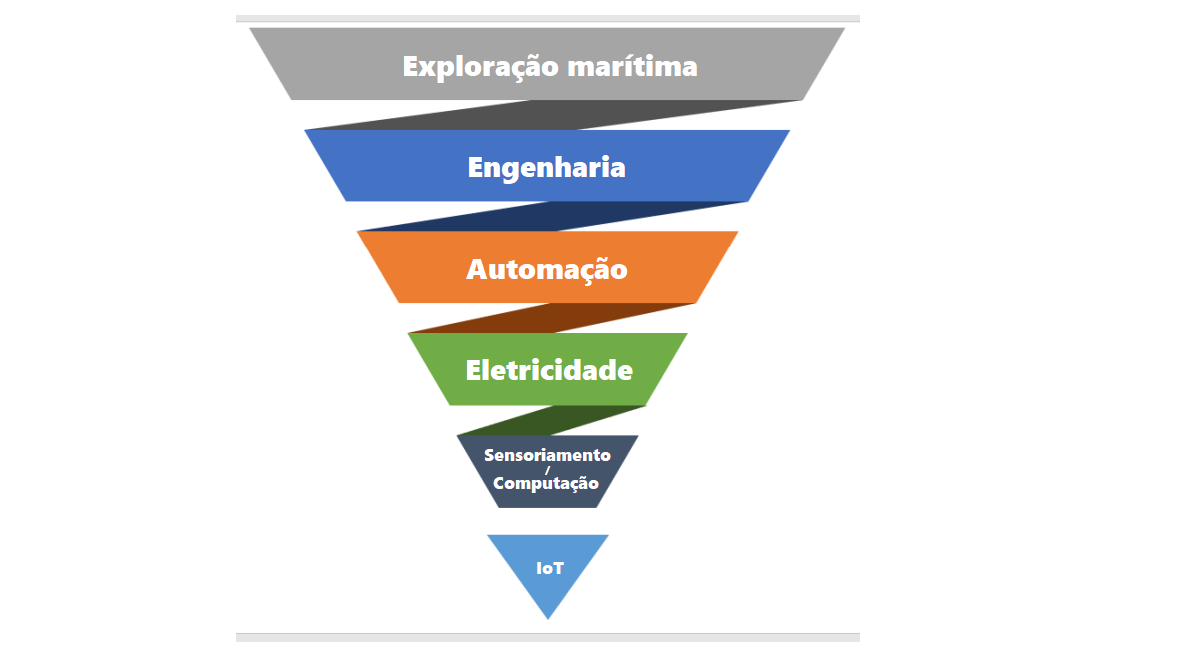
\includegraphics[width=16cm]{figuras/Datta.png}
    \fonte{Retirado de \textcite{datta2017}.}
  \end{varwidth}
\end{figure}

\section{Protocolo HTTP}
De acordo com \textcite{RFC2616}, o HTTP é um protocolo de comunicação utilizado para sistemas de informação distribuídos e colaborativos. Ele foi concebido para possibilitar a comunicação entre clientes e servidores na Rede Mundial de Computadores - WWW (sigla do inglês, \textit{World Wide Web}).

O HTTP foi introduzido em 1989 por Tim Berners-Lee enquanto ele trabalhava na Organização Europeia para a Pesquisa Nuclear - CERN (sigla do francês, \textit{Conseil Européen pour la Recherche Nucléaire}). A necessidade premente de compartilhar e distribuir informações de forma eficiente em uma rede de computadores motivou o desenvolvimento desse protocolo, que se tornou fundamental para a \textit{web} moderna \parencite{Berners_web}. Ele pode ser definido como:

\begin{quote}
"Um protocolo de camada de aplicação que define a estrutura de mensagens trocadas entre clientes e servidores. Ele opera sobre o Protocolo de Controle de Transmissão/Protocolo de Internet (TCP/IP), permitindo, nesta instância, a solicitação e transferência de recursos, como documentos HTML, imagens e vídeos, pela web." \parencite[{p. 7}]{RFC2616}
\end{quote}

No âmbito do desenvolvimento de sistemas, o HTTP desempenha um papel importante na criação de Interfaces de Programação de Aplicativos - APIs (sigla do inglês, \textit{Application Programming Interfaces}), possibilitando a comunicação entre diferentes componentes. Os desenvolvedores têm a capacidade de criar pontos de acesso HTTP que aceitam solicitações e respondem com dados formatados, como JSON ou XML \parencite{Newmann_web}.

Na Tabela \ref{tab:metodos_http} são destacados os principais métodos de solicitação do HTTP, utilizados para a interação entre clientes e servidores. No cotidiano, esses métodos são usados para a obtenção de informações, o envio de dados e a execução de operações em sistemas distribuídos, como aplicações \textit{web} e APIs.

Contudo, por si só, o HTTP não é adequado para aplicações da IoT, devido à sua natureza orientada a texto e ao alto consumo de largura de banda \parencite{Yassein_mqtt2017}. Para esses casos, o protocolo MQTT é mais adequado, como será abordado na próxima subseção.

\begin{table}[!htb]
  \caption{Métodos HTTP} \label{tab:metodos_http}
  \begin{tabularx}{\textwidth}{|c|X|} \hline
    \textbf{Método} & \textbf{Descrição} \\ \hline
    GET & Solicita a representação de um recurso específico. \\ \hline
    POST & Envia dados para serem processados por um recurso identificado no servidor. \\ \hline
    PUT & Substitui todas as representações atuais do recurso de destino com os dados enviados na solicitação. \\ \hline
    DELETE & Remove o recurso identificado no URI. \\ \hline
    PATCH & Aplica modificações parciais a um recurso. \\ \hline  
  \end{tabularx}
  \fonte{Adaptado de \textcite{RFC2616}.}
\end{table}

\section{Protocolo MQTT}

O MQTT foi introduzido pela primeira vez em 1999 por Dr. Andy Stanford-Clark, da IBM, e Arlen Nipper, da Arcom (agora Eurotech) \parencite{Yassein_mqtt2017}. Segundo \textcite{Andy_mqtt2004}, o MQTT foi inicialmente desenvolvido para o monitoramento de oleodutos e gasodutos através de comunicações de telemetria. Ele é definido como:

\begin{quote}
"Um método de transporte de dados leve para publicação e assinatura sobre TCP/IP com várias garantias de entrega. Otimizado para uso mínimo de largura de banda de rede e facilidade de implementação em sistemas embarcados, ele serve como um mecanismo de transporte onde é possível decidir o que enviar e quais ações tomar ao receber os dados." \parencite[{p. 4}]{Andy_mqtt2004}
\end{quote}

Nos sistemas embarcados, o MQTT é implementado nos dispositivos para permitir a troca de dados \parencite{Andy_mqtt2004}. Os dispositivos podem publicar dados de sensores e \textit{status} usando tópicos MQTT, enquanto as aplicações podem se inscrever nesses tópicos para receber e processar os dados em tempo real \parencite{Yassein_mqtt2017}.

Do lado do servidor, os \textit{brokers} MQTT são implantados para gerenciar a troca de mensagens entre os dispositivos e as aplicações. Segundo \textcite{Yassein_mqtt2017}, esses \textit{brokers} são responsáveis por rotear as mensagens entre os clientes MQTT, garantindo a entrega dos dados. Além disso, os desenvolvedores podem usar bibliotecas MQTT em suas aplicações para se conectar aos \textit{brokers}, facilitando a implementação de funcionalidades de comunicação em seus sistemas \parencite{MQTT_org}.

Em sistemas IoT, o MQTT é utilizado para conectar dispositivos a plataformas de nuvem, permitindo o monitoramento e controle remoto dos dispositivos \parencite{junior2022data}. As aplicações podem processar os dados recebidos dos dispositivos IoT, realizar análises em tempo real e realizar ações com base nos eventos detectados \parencite{ferrandez2018precision,hsu2020creative}. Suas principais características são definidas na Tabela \ref{tab:caract_mqtt}.

A implementação de sistemas de IoT na zona rural enfrenta desafios devido à baixa disponibilidade de internet e eletricidade na maioria dos casos \parencite{rijswijk2021digital}. No entanto, o MQTT se destaca como uma solução para esses cenários. Ele oferece uma comunicação assíncrona entre dispositivos, reduzindo a dependência de conexões de alta velocidade e garantindo a entrega de mensagens \parencite{Andy_mqtt2004, Yassein_mqtt2017}. Essa característica o torna uma opção para superar limitações de infraestrutura em áreas remotas. 

Sua eficiência o posiciona como uma ferramenta para a agricultura inteligente \parencite{Gurjeet_smart2022}, tema que será discutido na próxima subseção.

\begin{table}[!htb]
  \caption{Características do protocolo MQTT} \label{tab:caract_mqtt}
  \begin{tabularx}{\textwidth}{|c|X|} \hline
    \textbf{Característica} & \textbf{Descrição} \\ \hline
    Leve & É leve e eficiente em termos de largura de banda e recursos de hardware. \\ \hline
    Assíncrono & Dispositivos podem enviar e receber mensagens de forma independente, sem bloqueio ou espera ativa. \\ \hline
    Padrão aberto & É um protocolo aberto e bem documentado. \\ \hline
    Qualidade de Serviço (QoS) & Oferece três níveis de QoS para garantir a entrega confiável das mensagens: QoS 0 (entrega no máximo uma vez), QoS 1 (entrega pelo menos uma vez) e QoS 2 (entrega exatamente uma vez). \\ \hline
    Tópicos & Usa um modelo de publicação/assinatura, onde os dispositivos podem publicar mensagens em tópicos específicos e se inscrever para receber mensagens de tópicos de interesse. \\ \hline  
    Baixa latência &  É projetado para minimizar a latência de rede, tornando-o adequado para casos de uso em tempo real, como telemetria, monitoramento e controle remoto. \\ \hline
    Segurança & Suporta autenticação e criptografia. \\ \hline
    Retenção de mensagens & Permite que o broker MQTT retenha as últimas mensagens publicadas em um tópico. \\ \hline  
  \end{tabularx}
  \fonte{Adaptado de \textcite{MQTT_org}.}
\end{table}

\section{Agricultura inteligente}
A agricultura passou por uma transformação impulsionada pelo advento das tecnologias digitais, marcando a era da agricultura inteligente. 

\begin{quote}
  "Também conhecida como agricultura 4.0 ou agricultura digital, é a próxima fase da agricultura industrial, impulsionada pela integração de tecnologias na agricultura." \parencite[{p. 424}]{Gurjeet_smart2022}
\end{quote}

Essa mudança de práticas agrícolas tradicionais para agricultura inteligente tornou-se imperativa. Ela é caracterizada pela integração de tecnologias emergentes, como a IoT, Análise de Dados em Grande Escala - BDA (siga do inglês, \textit{Big Data Analysis}), computação em nuvem e IA. Seu objetivo é atender às crescentes demandas por segurança alimentar em uma população global em rápido crescimento \parencite{Gurjeet_smart2022, Garg_smart2023}.

Segundo \textcite{Garg_smart2023}, a convergência dessas tecnologias possibilitou o paradigma da agricultura orientada por dados, onde a coleta, análise e tomada de decisões em tempo real são centrais para otimizar práticas agrícolas.

\textcite{Gurjeet_smart2022} complementa que, ao elucidar o estado atual da adoção de tecnologia digital na agricultura e identificar perspectivas futuras, são abertos caminhos para práticas agrícolas sustentáveis e eficientes.

A agricultura inteligente, ao incorporar IA e análise avançada de dados, busca orientar decisões mais adaptativas e holísticas \parencite{Garg_smart2023}. Para isso, é necessário a coleta e aplicação precisa de dados para otimizar a produção \parencite{Lamine_precision2024}, a qual será abordada na próxima subseção.

\section{Agricultura de precisão}

A agricultura de precisão pode ser definida como: 

\begin{quote}
  "A aplicação de tecnologias e princípios para gerenciar a variabilidade espacial e temporal associada a todos os aspectos da produção agrícola com o propósito de melhorar o desempenho das culturas e a qualidade ambiental." \parencite[{p. 1}]{Pierce_precision1999}
\end{quote}

Segundo \textcite{Pierce_precision1999}, o sucesso da agricultura de precisão está relacionado à sua capacidade de avaliar e gerenciar o continuum espaço-tempo na produção de culturas. Ela é habilitada pela tecnologia e integrada por tecnologias específicas que permitem avaliar e gerenciar a variabilidade em níveis de detalhe nunca antes alcançados \parencite{Zhang_precision2002}. No entanto, o sucesso agronômico da agricultura de precisão tem sido limitado e inconsistente, embora bastante convincente em alguns casos, complementa \textcite{Zhang_precision2002}.

Atualmente, de acordo com \textcite{Lamine_precision2024}, a agricultura de precisão é uma prática que busca observar, medir e responder às variações que ocorrem dentro de um mesmo campo e entre diferentes campos. Isso significa identificar as diferenças no solo, nas plantas e nas condições ambientais, tanto dentro de uma área de cultivo quanto entre áreas agrícolas distintas. Ao entender essas variações, é possível adotar abordagens específicas para cada local. Exemplo disso é ajustar a quantidade de fertilizantes ou de água, o que torna a produção mais eficiente e contribui para a conservação ambiental \parencite{Lamine_precision2024}.

Apesar dos avanços tecnológicos e inovações, a agricultura de precisão ainda enfrenta desafios em países em desenvolvimento, especialmente em agricultura de pequena escala, conforme apontado por \textcite{Lamine_precision2024}. No entanto, existem amplas oportunidades e perspectivas para a adoção de inovações em agricultura de precisão \parencite{Lamine_precision2024}.

A agricultura de precisão compreende um conjunto de tecnologias que combinam sensores e sistemas de informação. Essas tecnologias são utilizadas para otimizar a produção, levando em consideração a variabilidade e as incertezas dentro dos sistemas agrícolas. Ela fornece meios para monitorar a cadeia de produção de alimentos e gerenciar tanto a quantidade quanto a qualidade dos produtos agrícolas \parencite{Gebbers_precision2010}.

\textcite{Francisco_precision2024} demonstraram que a avaliação do ciclo de vida de tecnologias de agricultura de precisão possui potencial para melhorar a sustentabilidade agrícola, embora seu impacto ambiental exato permaneça incerto. Estudos comparativos mostraram que a agricultura de precisão pode reduzir os impactos ambientais da produção agrícola, especialmente no que diz respeito à gestão da irrigação \parencite{Francisco_precision2024}. No entanto, é importante considerar variáveis locais para uma avaliação ambiental abrangente, como será abordado na próxima subseção.

\section{Gestão da irrigação}

\textcite{Burton_irrigation2010} apresenta a gestão eficaz da irrigação como um desafio que demanda pesquisas e práticas sustentáveis, juntamente com o uso de tecnologias apropriadas. 
Considerando a complexidade das demandas e ofertas de recursos hídricos em perímetros irrigados, é essencial a utilização de técnicas e instrumentos para auxiliar profissionais nesse processo \parencite{Ramos_irrigacao2022}. Neste contexto, é fundamental o conhecimento da variabilidade espacial dos atributos do solo. Segundo \textcite{Ramos_irrigacao2022}, essa variabilidade está relacionada ao fluxo e armazenamento de água, usados como parâmetros para a otimização da produção agrícola.

\textcite{Pereira_irrigation2002} discutem diversos aspectos relacionados à gestão da irrigação em propriedades agrícolas, incluindo o uso de águas residuais tratadas e águas salinas. Os autores destacam a importância de estratégias como a uniformidade de distribuição e práticas de irrigação suplementar e deficitária para reduzir a necessidade de água na agricultura.

O estudo conduzido por \textcite{Burton_irrigation2010} complementa essas discussões. Ele destaca a importância das tecnologias, tais como o sensoriamento e a telemetria das condições ambientais, na agricultura irrigada. Além disso, ressalta a necessidade de desenvolver metodologias capazes de avaliar os benefícios sociais, econômicos e ambientais resultantes da otimização desse processo.

A integração dessas estratégias e tecnologias possibilita uma gestão mais eficiente da irrigação em áreas específicas, onde o consumo hídrico é variável \parencite{carmody_fao2023}. Essa integração, aliada a espacialização dos dados, apresenta melhorias efetivas do uso da água em escalas, como a de um perímetro irrigado \parencite{Burton_irrigation2010, Ramos_irrigacao2022}. Na próxima subseção, será discutida uma das perspectivas da gestão hídrica na agricultura relevante para este trabalho.

\subsection{Gestão baseada no consumo de água}

Segundo \textcite{carmody_fao2023}, a gestão baseada no consumo de água traz uma perspectiva inovadora. Ela considera não apenas a entrega de água, mas também o uso real da mesma na agricultura. Isso contribui para a eficiência do uso dos recursos hídricos e para a sustentabilidade dos sistemas agrícolas. 

Na Figura \ref{figura:ciclo_agua}, é apresentado o ciclo da água. Ele é definido como um processo contínuo que envolve a precipitação, infiltração, evaporação, evapotranspiração (ET) e condensação \parencite{carmody_fao2023}. A água precipitada em forma de chuva ou neve alimenta os reservatórios superficiais e subterrâneos. Parte dela infiltra-se no solo, recarregando os lençóis freáticos, enquanto outra parte escoa superficialmente, mantendo o fluxo de rios e riachos. A evaporação dos corpos d'água e a ET das plantas retornam a umidade à atmosfera, onde se condensa formando nuvens, completando o ciclo.

Neste modelo, a água pode ser utilizada de duas formas: benéfica, como na transpiração das plantas para a produção de alimentos, e não benéfica, como na evaporação do solo nu ou de superfícies de água nuas. Também existem os fluxos de retorno não consumidos, que podem ser recuperados para consumo benéfico ou para manter os ecossistemas aquáticos (Figura \ref{figura:ciclo_agua}). Eles contribuem para o abastecimento de outros usuários a jusante e para a saúde dos rios e lençóis freáticos \parencite{carmody_fao2023}.

De acordo com \textcite{carmody_fao2023}, para alcançar economias reais de água, é necessário atender a quatro requisitos no contexto de um quadro mais amplo. Nesse quadro, os fluxos ambientais são considerados para sustentar os sistemas agrícolas e as pessoas que dependem deles. Esses requisitos incluem:

\begin{enumerate}
\item A determinação dos requisitos específicos de ET para a produção de culturas;
\item A definição dos direitos de água em termos de extração, consumo e fluxos de retorno;
\item O uso do monitoramento de ET e cobertura do solo para ajustar as alocações de água;
\item A comparação da ET alvo com a ET real para garantir um balanço hídrico adequado.
\end{enumerate}

Para compreender a ET e sua importância na gestão da água, é necessário analisar o cenário em que a mesma surge, como será abordado na próxima subseção.

\begin{figure}[!htb] \centering
  \caption{Ciclo Hidrológico} \label{figura:ciclo_agua}
  \begin{varwidth}{\linewidth}
    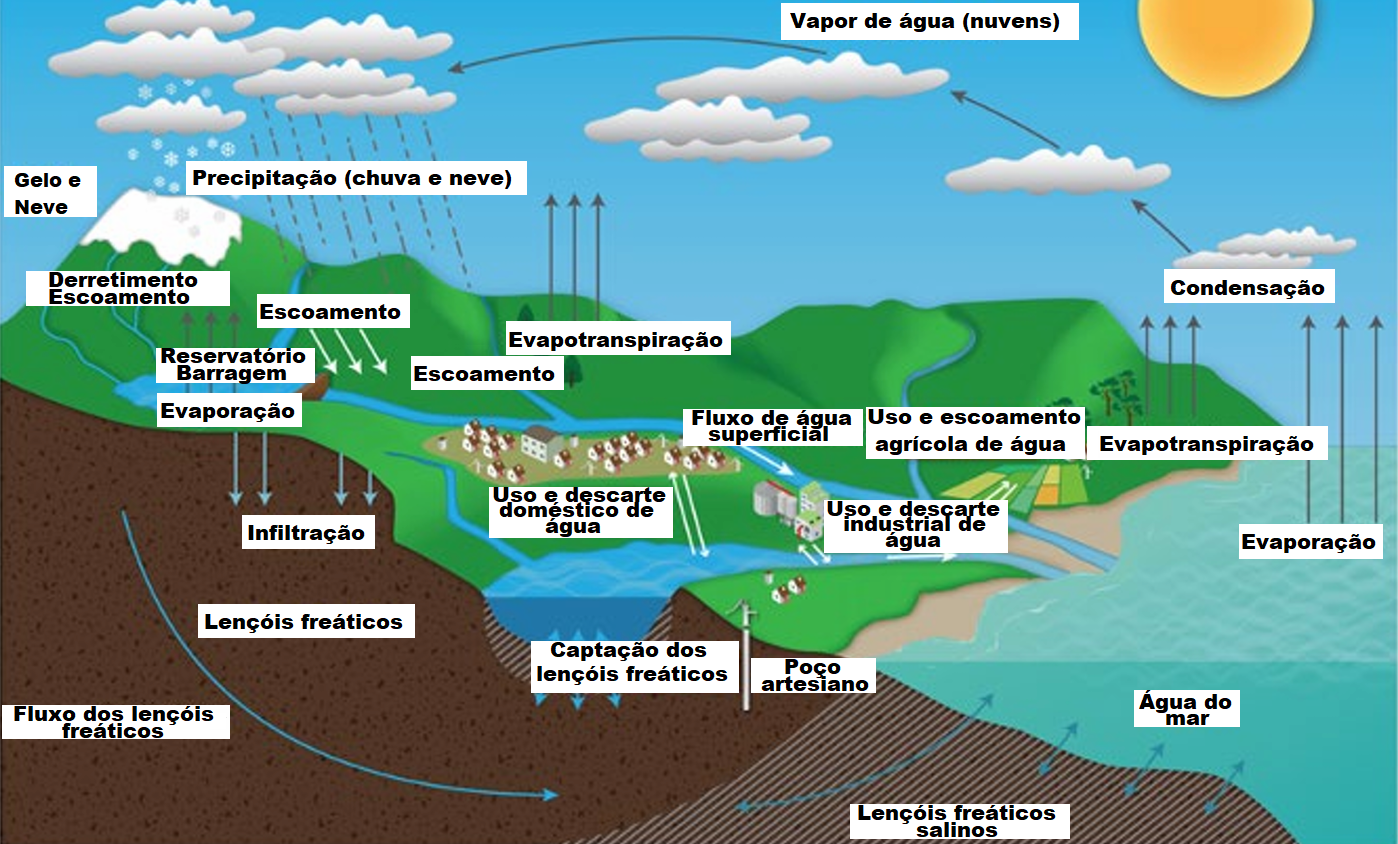
\includegraphics[width=16cm]{figuras/Carmody.png}
    \fonte{Retirado de \textcite{carmody_fao2023}.}
  \end{varwidth}
\end{figure}

\section{Evapotranspiração}

A ET descreve o processo fundamental de transferência de água da superfície da Terra para a atmosfera \parencite{carmody_fao2023}. A ET desempenha um papel importante na dinâmica hídrica. Foi observado que:

\begin{quote}
  "Três tipos de superfície são importantes no retorno da chuva à atmosfera. Para extensas áreas de terra, são eles, em ordem de importância: vegetação, na qual as folhas das plantas atuam como superfícies transpirantes; solo nu ou pousio, de onde a água evapora na interface solo-ar ou logo abaixo dela e em águas abertas, a partir das quais a evaporação ocorre diretamente." \parencite[{p. 121}]{Penman_evapotranspiration1948}
\end{quote}

\textcite{Penman_evapotranspiration1948} explica que a irrigação exerce uma influência direta na evaporação ao fornecer água ao solo. Esse processo não apenas afeta a disponibilidade de água para a evaporação, mas também influencia a temperatura e a umidade do solo, fatores determinantes para a taxa de ET. As interações entre a atividade humana e os ciclos naturais da água são particularmente relevantes no contexto das mudanças climáticas globais. 

Conforme destacado por \textcite{yang_nature2023}, tem-se observado uma tendência de aceleração no aumento da ET desde a década de 1980. Essa tendência está intimamente ligada à expansão da vegetação e ao aumento da área plantada, o que é evidenciado pelo crescimento do índice de área foliar (LAI).

O aumento da ET pode ter consequências tanto positivas quanto negativas. Por um lado, pode indicar um crescimento saudável da vegetação, o que pode ser benéfico para a agricultura e para a absorção de carbono. Por outro lado, um aumento excessivo da ET pode resultar em uma maior demanda por água, potencialmente levando ao estresse hídrico, especialmente em regiões onde a disponibilidade de água é limitada. \textcite{yang_nature2023} indicam a mensuração da ET para avaliar os impactos das atividades antropogênicas no ciclo hidrológico e no clima.

Métodos de telemetria da ET têm mostrado resultados promissores na compreensão desse fenômeno em escalas regional e global. De acordo com as revisões feitas por \textcite{Zhao_evapotranspiration_med2009, Zhang_evapotranspiration_med2016}, esses métodos variam desde modelos de equações simplificadas até modelos de balanço energético de duas fontes mais complexos. 

Segundo \textcite{Zhao_evapotranspiration_med2009}, os modelos mais eficazes utilizam sensores telemétricos que capturam a radiação emitida pelo solo, cobrindo desde o espectro visível até o infravermelho térmico. Essa abrangência espectral permite uma estimativa precisa da radiação líquida, um dos principais componentes do balanço de energia da superfície \parencite{Zhao_evapotranspiration_med2009}. No entanto, há uma dependência, em certa medida, de medições auxiliares baseadas em solo para derivar os fluxos de calor turbulentos em uma escala regional \parencite{Zhang_evapotranspiration_med2016}.

O coeficiente de determinação (\(R^2\)) é uma medida estatística que indica a proporção da variabilidade dos dados explicada pelo modelo \parencite{mood1974}. Ele é calculado pela fórmula:

\[
R^2 = 1 - \frac{\sum_{i=1}^n (y_i - \hat{y}_i)^2}{\sum_{i=1}^n (y_i - \bar{y})^2}
\]

\noindent em que: \(y_i\) são os valores observados, \(\hat{y}_i\) são os valores previstos pelo modelo e \(\bar{y}\) é a média dos valores observados. O valor de \(R^2\) varia de 0 a 1, onde um valor próximo de 1 indica que o modelo explica a maior parte da variação nos dados. \textcite{Yang_evapotranspiration_med2022} apresenta um método de telemedição de ET com coeficiente de determinação de 0,88. Neste estudo, a fusão de dados de diferentes satélites (Landsat 8 e Sentinel-2) com resoluções espaciais e temporais variáveis proporciona uma estimativa contínua e precisa da ET diária em escala de campo.


Plataformas como o \textit{USGS EarthExplorer} e o \textit{Copernicus Open Access Hub} possuem acesso aberto as imagens dos satélities citados com alta resolução. Essas imagens serão utilizadas para a obtenção de dados no presente trabalho.

Nas duas próximas subseções, serão abordados conceitos e técnicas complementares as definições apresentadas acima, que serão de utilidade para o desenvolvimento do sistema proposto.

\subsection{Evapotranspiração de referência}

A ET de referência (ETo) é definida como:

\begin{quote}
  "A taxa de evapotranspiração de uma superfície de referência, sem falta de água." \parencite[{p. 7}]{Allen_evapotranspiration1998}
\end{quote}

Para calcular a ETo, pode-se empregar o método da FAO-56 apresentado por \textcite{Allen_evapotranspiration1998}, uma abordagem recomendada pela Organização das Nações Unidas para Alimentação e Agricultura, que é definida pela equação:

\begin{equation}
ETo = \frac{0.408 \cdot \Delta (R_n - G) + \gamma \cdot \frac{900}{T + 273} \cdot u2 \cdot (e_s - e_a)}{\Delta + \gamma \cdot (1 + 0.34 \cdot u2)}
\end{equation}

\noindent em que: ETo é a evapotranspiração de referência; $R_n$ é a radiação líquida; $G$ é o calor do solo; $\Delta$ é o déficit de pressão de vapor; $\gamma$ é a constante psicrométrica; $T$ é a temperatura média do ar; $u2$ é a velocidade do vento a 2 metros de altura; $e_s$ é a pressão de vapor do ar saturado; $e_a$ é a pressão de vapor do ar.

\subsection{Evapotranspiração de cultura}

A ET de cultura (ETc), por sua vez, é definida como:

\begin{quote}
  "A evapotranspiração de culturas livres de doenças, bem fertilizadas, cultivadas em grandes campos, sob condições ótimas de água no solo e atingindo plena produção nas condições climáticas dadas." \parencite[{p. 7}]{Allen_evapotranspiration1998}
\end{quote}

A ETc pode ser calculada como o produto da ETo e um determinado coeficiente de cultura (Kc), como proposto por \textcite{Allen_evapotranspiration1998}:

\begin{equation}
ETc = Kc \cdot ETo
\end{equation}

O Kc é um fator que leva em consideração as características específicas da cultura, como a fase de desenvolvimento, a densidade de plantio e a cobertura do solo. Ele é determinado experimentalmente e varia ao longo do ciclo de cultivo \parencite{bernardo_irrigacao2008}.

A determinação da ETc em tempo real é um dos principais objetos de estudo dessa pesquisa. Na próxima seção, serão apresentados trabalhos similares e como a proposta deste trabalho se diferencia deles.

\section{Revisão bibliográfica}

O monitoramento da ETc é uma prática que possui diversas abordagens e métodos, dependendo do ambiente e do nível de precisão desejado. A ETc pode ser estimada por meio de métodos diretos, como a pesagem de lisímetros, ou indiretos, como a equação de \textcite{Allen_evapotranspiration1998} apresentada na seção anterior. Entre essas abordagens, esta pesquisa propõe uma aplicação \textit{web} para o monitoramento da ETc em tempo real, combinando métodos indiretos para esse fim.

A seguir serão apresentados outros trabalhos com abordagens semelhantes.

\subsection{Integração de dados e padrões \textit{web} para modelos de ETo}

\textcite{Jianting_webeva2009} abordam o desenvolvimento de sistemas de disseminação de dados em tempo real baseados na aquisição de dados. Eles fazem uso de dados geoespaciais para estimar a ETo diária, apontando a necessidade de métodos de acesso públicos a esses dados. Isso contrasta com os métodos utilizados nos serviços existentes com o mesmo propósito.

Os autores desenvolveram um sistema que utiliza padrões da \textit{Open Geospatial Consortium} (OGC) e o protocolo \textit{Network Data Access Protocol} (OPeNDAP) para publicar dados de estações meteorológicas. A arquitetura desse sistema incorpora diversas fontes de dados distribuídas e heterogêneas, como registros diários e horários de estações geoestacionárias. Além disso, imagens de satélite e resultados de modelos meteorológicos são utilizados para uma análise espacial. 

Através de serviços construídos sobre essas fontes, o sistema prova a eficácia de uma abordagem distribuída. Isso permite tanto a utilização quanto o desenvolvimento de novos serviços e aplicações sem interferir nos já existentes.

O trabalho de \textcite{Jianting_webeva2009} promove várias vantagens em relação à interoperabilidade e padronização de dados. No entanto, esse método não considera medições realizadas diretamente no local de interesse (\textit{in situ}). Isso, em cenários menores, como o de uma propriedade rural, pode ser uma limitação em questão de precisão e custo. Além disso, o sistema proposto não oferece uma interface para a visualização e análise dos dados, o que pode dificultar a interpretação dos resultados por usuários finais.

\subsection{Ferramentas \textit{web} para determinação de ETo}

O estudo de \textcite{Fangming_webeva2021} foca no desenvolvimento e implementação de APIs em nuvem, chamadas \textit{ETWatch}, para a geração de dados regionais da ETo. Essas APIs são desenvolvidas para proporcionar acesso fácil e em tempo real aos dados de ETo.

A metodologia combina dados de sensoriamento remoto, medições \textit{in situ} e modelagem matemática para calcular a evapotranspiração. As APIs facilitam a disseminação desses dados para diversos usuários e aplicações. Entre as vantagens do sistema \textit{ETWatch}, destacam-se o acesso em tempo real aos dados de ETo, permitindo uma resposta rápida para a gestão de recursos hídricos. Além disso, o sistema fornece uma interface para monitorar os dados, facilitando o acesso e a leitura das informações obtidas.

Apesar das vantagens, \textcite{Fangming_webeva2021} identificam alguns pontos que necessitam de maior preocupação. A precisão das estimativas pode ser limitada pela qualidade e disponibilidade dos dados de entrada, especialmente em regiões com poucas medições \textit{in situ}. A complexidade de integrar modelos climáticos e hidrológicos pode apresentar desafios computacionais e de implementação. Além disso, há a necessidade de ajustar os modelos para responder a variações e mudanças climáticas contínuas.

Uma abordagem semelhante foi realizada por \textcite{Jose_webeva2011} com o desenvolvimento de uma aplicação \textit{desktop} chamada \textit{CropWaterUse}. Essa aplicação foi desenvolvida para estimar os tempos de irrigação baseados na estimativa de ETc. Assim como \textcite{Fangming_webeva2021}, \textcite{Jose_webeva2011} utilizaram medições e modelos matemáticos para estimar a ETo. Contudo, eles realizaram o cálculo da ETc com base na ETo e em valores de Kc específicos para cada cultura, sendo estes inseridos manualmente pelo usuário na aplicação.

Porém, a aplicação \textit{CropWaterUse} não oferece uma interface de acesso distribuído para a visualização dos dados, seja por meio de APIs ou nuvens de dados. Isso limita sua utilização em cenários remotos ou até mesmo restritos, como propriedades rurais.

\subsection{Desenvolvimento e aplicação de ferramentas para ETo}
No estudo de \textcite{Taison_webeva2019}, foi desenvolvido um sistema que automatiza o cálculo da ETo, integrando dados de estações meteorológicas e métodos matemáticos. Diferente das pesquisas apresentadas, esse sistema adota o padrão de arquitetura \textit{Model-View-Controller} (\textit{MVC}) para o projeto. Esse \textit{design} separa a lógica de negócio, definida como \textit{Model}, da interface gráfica, chamada de \textit{View}. O \textit{Controller} é responsável por intermediar a comunicação entre o \textit{Model} e a \textit{View}. Dessa forma, é possível desacoplar as camadas do sistema, facilitando a manutenção e a evolução do mesmo.

A aplicação de \textcite{Taison_webeva2019} é eficiente quanto a interface e a arquitetura. No entanto, o sistema não considera medições \textit{in situ} para o cálculo da ETo, o que pode limitar a precisão dos resultados para pequenas áreas como já mencionado. 

Uma abordagem que contorna esse problema é apresentada por \textcite{Serban_webeva2022}. Ele destaca a criação e funcionalidade do \textit{ETCalc}, uma ferramenta gratuita para estimativa de ETo. Seu diferencial está na possibilidade de fornecer dados meteorológicos de múltiplas fontes. Ele permite que os usuários calculem a ETo em suas propriedades, com base em dados fornecidos de estações e medições locais. O \textit{ETCalc}, dentre as pesquisas encontradas, é a aplicação que possui o processamento matemático mais robusto, considerando diferentes métodos e parâmetros. Também fornece uma interface para a inserção e visualização dos dados, facilitando o acesso e o uso da ferramenta.

Apesar das vantagens, o \textit{ETCalc} falha como processo automatizado e em tempo real. O usuário precisa inserir manualmente os dados de entrada, o que pode ser um processo demorado e propenso a erros. Além disso, a ferramenta não oferece APIs para a integração com outros sistemas, o que limita sua utilização em cenários mais complexos.

Com base nas pesquisas apresentadas, na tabela \ref{tab:comparacao}, é possível observar as tecnologias e métodos utilizados em cada uma delas. Também é possível identificar as limitações de cada abordagem, que servirão de base para o desenvolvimento da aplicação proposta nesta pesquisa.

\begin{table}[!htb]
    \caption{Comparação das tecnologias} \label{tab:comparacao}
    \begin{tabularx}{\textwidth}{|X|X|X|} \hline
        \textbf{Referência} & \textbf{Tecnologias} & \textbf{Limitações} \\ \hline
        \textcite{Taison_webeva2019} & \textit{PHP}, \textit{Smarty Template Engine}, \textit{HTML5}, \textit{CSS3}, \textit{JavaScript}, \textit{Bootstrap}, \textit{OpenLayers} e \textit{PostgreSQL}. & Escalabilidade limitada e performance inferior em aplicações complexas. \\ \hline
        \textcite{Serban_webeva2022} & \textit{Python}, \textit{Django}, \textit{HTML5}, \textit{CSS3}, \textit{JavaScript}, \textit{jQuery}, \textit{Bootstrap} e \textit{PostgreSQL}. & Menor performance em aplicações de alta carga e necessidade de alto conhecimento técnico em \textit{Python}. \\ \hline
        \textcite{Jose_webeva2011} & \textit{C\#}, \textit{ASP.Net}, \textit{Visual Studio.NET}, \textit{JavaScript}, \textit{TeeChart} e \textit{SQL Server}. & Dependência de plataforma \textit{Windows} e custos elevados de licenciamento. \\ \hline
        \textcite{Fangming_webeva2021} & \textit{Python}, \textit{Bootstrap}, \textit{jQuery}, \textit{Alibaba Cloud}, \textit{IDL}, \textit{Docker}, \textit{JSON} e \textit{PostgreSQL}. & Complexidade na integração e maior curva de aprendizado para configuração. \\ \hline
        \textcite{Jianting_webeva2009} & \textit{OGC standards}, \textit{OPeNDAP standards}, \textit{WMS}, \textit{WCS}, \textit{WFS}, \textit{GIS}, \textit{DODS}, \textit{DAS}, \textit{DDS} e \textit{Middleware components}. & Alta complexidade de implementação e necessidade de especialização em padrões \textit{OGC}. \\ \hline
        Presente pesquisa & \textit{C}, \textit{Node.js}, \textit{Next.js}, \textit{Shadcn/ui}, \textit{Tailwind CSS} e MQTT. & Alto consumo de memória em aplicações de alta carga e maior curva de aprendizado inicial para integração do MQTT. \\ \hline
    \end{tabularx}
    \fonte{Elaborado pelo autor, 2024.}
\end{table}
